% 来源：OEBPS/Text/Section0001_split_008.xhtml#sigil_toc_id_58

\BookChapter{44}
\section[第44章\q 未来比你想象的更加光明]{第44章\\ 未来比你想象的更加光明}

\begin{BookQuote}
生活的关键是，要相信最好的还在后面。

\hfill ——彼特·乌斯蒂诺夫
\end{BookQuote}

为什么大多数人要追逐财富？因为他们要追逐更高品质的生活。毋庸置疑，那就是任何人都能够应对艰难的日子，只要可以确定有更好的明天。

我们都需要美好的未来。

你是否在疑惑，为什么我写的是一本投资理财书，却要花时间大谈未来和科技上的突破创新，这是因为科技是一种隐藏的资产，每一天科技水平都在呈复利式增长，让我们的生活更加富足。

每天都在发生颠覆性创新，未来几个月、几年，将会发生革命性的创新，以提高你和地球上所有人的生活品质，这种高科技的发展进步像巨大的浪潮，让我们所有人像船一样都向上浮，生活品质大大提高。

用金融术语来讲，你知道科技创新最厉害的地方是什么吗？科技创新的成本在减少，而科技创新的能力在呈指数化扩大！你知道这对于你来说意味着什么吗？这意味着即使你现在才开始打造财富，即使年纪已相当大而财富一点儿都不多也没关系，你将来还是能够拥有品质很高的生活，所需要的钱比你想的还要少。

而且，学习了解这些高科技发展的趋势，能够让你清醒地意识到，你这一生正面临最伟大的投资机会。这些科技创新正在呈指数化增长。你要留意关注这些科技创新，时间就从现在开始。

我希望这一章的内容能够激励你更好地照顾自己和你的家人，不仅是在财务上，还要在身体上。没有健康的身体，就没有财富。你要活得时间足够久，才能充分利用科技上的巨大进步，你应该把健康长寿放在第一位，特别是你听我下面讲到有些巨变正在展开之后，更要把健康放在第一位。

让我们来展开一段简短的科技最前沿之旅，探索科技未来发展的最前沿。我要先说一下，这一章的内容是一点儿也不怕出错的积极观点，这并不是基于我个人的热情，而是反映了目前世界上一些伟大科学家做的研究工作成果。这些人，不是只会预测，而是亲自把自己的预测变成现实成果。这些人已经做了很多了不起的大事：解码人类基因，设计出第一个数字语音识别系统，设计研发商业运载火箭以实现载人在地球和国际空间站之间往返运输。

我知道，很多人对科技创新的观点和我不同，有很多怀疑。也许他们是对的。有些人展望未来，看到的是像电影《终结者》那种类型的机器人杀手，还有转基因食品。有些人展望未来，看到的是：会飞的汽车，就像动画片《杰森一家》里的一样；灵活的机器人帮手，像电影《星球大战》中的C–3PO一样的人形机器人助手；肉和蔬菜可以从单细胞培养出来以提高生产效率，完全可以解决世界饥饿问题。不过所有这些极端的未来场景，没有一个变成现实。所以我选择探索的问题更加实用一些，如何利用科技创新大幅度提升我们的生活品质，更健康，更美好。我知道，人们往往对科技创新出来的新东西感到恐惧，担心我们发展得实在太快了。

毕竟这些科技进步都有负面影响，通常是因为这些科技一开始会让人们丢掉原来熟悉的工作，直到他们适应新技术，学会用新方式工作，正如史蒂夫·拉特勒这位影响力很大的金融家和专栏作家在《纽约时报》上撰文所指出的那样，即使是英格兰伊丽莎白女王一世，也拒绝给一台16世纪的纺布机器颁发专利，因为这会让她那些“可怜的臣民”丢掉工作。但是按照拉特勒的看法：“这项科技创新并不是为了保住旧工作……而是为了创造新工作。自从车轮发明以来，就经常如此。”

大多数时候，这些新工具用以提升人的生活品质。但是现在世界面临一些巨大的挑战：过多的二氧化碳排放、缺少淡水、耕地短缺，而科技创新正在解决这些大难题。所有这些科技进步看起来好像一夜之间发生的，但是从整个历史来看，也有少数人会利用任何工具或者任何科学技术作为武器来危害人类。比如电力既可以用于路灯照明，也可以用于电椅杀人，但是世界上的路灯有好几百万个，数量要远远超过杀人的电椅。波音喷气式飞机既可以用来载人穿越大洋，也可以用来载着炸弹杀死成千上万人，但是世界上的民用航空飞机数量比战斗机多出好几百万架。

人类害怕新事物，未知的事物，过多关注最糟糕的情况以做最坏的打算，这很自然。我们的大脑天生是为了追求生存，我们作为一个物种天生就是这样的，把生存放在第一位。但是我们的想象力也可能会阻碍我们。科幻小说让很多人恐惧未来的科技发展，就像人工智能。但是现实派的科学家和未来学家，就像雷·库兹韦尔、彼得·戴曼迪斯、胡安·恩里奎，都是把先进的科技看作机会，它们能让人类进化得更好，让世界变得更好。

如果你一看未来如此积极乐观就怒了，你可以马上转到下一章！但是如果你真的对未来很感兴趣，想要知道科技如何塑造我们的生活，我想这一章肯定会帮助你明白，哪些科技就在身边可以使用，哪些正在到来。我看待科技的方式是，你可以选择恐惧未来，也可以拥抱未来。不管你怎么做，都不会改变科技，而科技肯定会改变你的生活。

为什么？因为未来已经来了。

\begin{BookQuote}
预测未来的最好方法就是创造未来。

\hfill ——艾伦·凯
\end{BookQuote}

每过10分钟，美国就有一个人严重烧伤。他们冲到医院，充满烧伤的痛苦——这是人体能够承受的最大痛苦。护士刮掉那些满是水疱和烧焦的皮肤，用从尸体上取下来的皮肤覆盖住伤口，以避免他们受到感染而死亡。你能想象吗？从尸体上取下来的皮肤盖在你自己的伤口上！即使伤者活下来，疤痕也非常严重。你会看到他们的脸上、胳膊上、腿上都是伤疤，面目全非。有的时候，需要进行多次手术，经过好多年才能痊愈。

那么你可以想象一下，有一天晚上，40多岁的州警马特·尤兰姆也被烧伤了，发现自己也成了这些残酷的统计数字中的一个。他的人生从此永远被改变了。

这是怎么回事？当时他坐在一堆篝火旁，有人往火里面扔了一罐汽油，结果大火燃烧起来，烧到了他的右臂、头、右脸。大家赶紧把他送到医院，医生和护士动作很快，清除掉起了水疱的皮肤，给伤口消毒，避免感染，涂了药膏。正常情况下，他应该在烧伤病房里住院几个星期，甚至好几个月，接受一系列痛苦的检查，每天两次。而这次不同于传统方式，有一个专家团队使用一种新的医疗科技为马特治疗。医疗专家从马特身上取下一小块没有烧伤的皮肤，得到了健康的皮肤细胞，而不是给马特使用从尸体上取下来的皮肤！医疗专家对这些细胞进行培养，不久之后，用喷枪喷到马特的伤口上，喷出来的都是马特自己的组织细胞溶液。

过了三天，马特的胳膊和脸上烧伤的皮肤就痊愈了。在马特身上几乎看不到任何伤疤。我知道这事听起来像是一个科幻片。但是这是一个真实的故事，几年前就发生在匹兹堡。

尽管治愈马特·尤兰姆烧伤的技术，在美国还处于临床实验阶段，但一个类似的干细胞手术已经在欧洲和澳大利亚用在几百个烧伤病人身上了。真让人吃惊，是不是？现在甚至有一种“生物笔”，能让外科医生从骨头和软骨不同层面上提取健康的细胞，这些细胞繁殖生长，成为神经、肌肉、骨骼，用来治愈受到损害的对应部分。科技能让外科医生把细胞置于他想要放的地方，一眨眼就能完成。这只是其中之一，还有好多不可思议的新型治疗方法正在投入使用，而且价格越来越便宜，人人都负担得起。

可能你还没有注意到：我们生活的这个世界，每一天都在发生奇迹，变化得非常快，有时我们甚至根本没有注意到。或者我们已经把这些变化看作理所当然。

但是如果你回到1980年，距离现在也不过是30多年前，你向那个时候的人描述我们现在的世界，他会觉得，你正在做的事情，简直是魔法一般不可思议！往皮肤上喷组织细胞？一边跟人打电话，一边开车？我的天哪，这简直太不可思议了。

我们习惯预测未来的方式是，看看今天发生了什么，或者昨天发生了什么，我们就能预测出明天会发生什么。但是再也不能这样预测未来。直到非常接近现在的“最近”，也是变化很少而且很慢的，可以用几十年甚至几百年的一个时代来衡量，比如铜器时代、铁器时代等。现在变化比过去快多了，而且是指数型加速变化。这意味着速度不是不变，而是快上加快，在很短的时间之内，就能发生巨大的跳跃性变化。这意味着，我们正在制造工具，把我们的生活品质改变得更快更好，现在这些工具每个人都能得到。

现在普通人都能享受到的东西，是古代最富有的帝王做梦都想不到的。想象一下，如果古代的帝王坐在椅子上或者躺在床上就能飞到天上，只用几个小时就能飞到世界上任何一个遥远的地方，而不是在海上航行好几个月才到达，那么这个帝王愿意给你多少金银财宝？现在，你只要付出494美元，坐上维珍·亚特兰大航空公司的飞机就能做到了。

即使是帝王，也不能花费2亿美元拍一部电影，娱乐自己2个小时。但是现在每个星期都有新电影上线，我们只要花上10美元就能在电影院看大片了，或者在视频网站上花9.99美元包月，大片随便看。

让我们面对现实吧，我们生活在地球上最非凡、最不可思议的时代。我们看到，最近100年，人类的寿命从30岁延长到67岁，寿命增加了1倍多。与此同时，全球平均收入增长了3倍。100年前，大多数美国人，只有每天把工作收入的43\%花在吃饭上，才能填饱肚子。现在，由于农业和物流分销的进步，现在美国人每天用在吃饭上的钱只占收入的7\%。

\subsection{你有新邮件}

我第一次见到美国前总统比尔·克林顿是在20世纪90年代早期，我还非常清楚地记得，我坐在他旁边对他说：“你看，总统先生，也许有个方法，能让我们用电子通信的方式沟通。”克林顿总统一听一脸迷惑，我马上解释说：“我已经开始使用这个新东西，它叫作电子邮件。我用美国在线开了电子邮件账户，你有吗？”克林顿总统说：“哦，我听说过那个东西！”但是那个时候，美国总统还没有电子邮件账户。现在亚马孙流域那些原始部落里的人，也带着手机在丛林里四处行走，他们的即时通信能力非常强大，35年前，连克林顿这个全世界最强大国家的领导人当时的即时通信能力也根本比不上。尽管住在丛林里，他也可以在线购买奶牛饮料，可以在线支付小孩的学费。他可以在线翻译，他愿意的话，甚至可以上耶鲁大学网站得到免费的经济学课程，也可以从麻省理工学院得到免费的数学课程。我们现在生活在一个完全不同的世界中，现在还只是在开始阶段。

\begin{figure}[htbp]
\centering
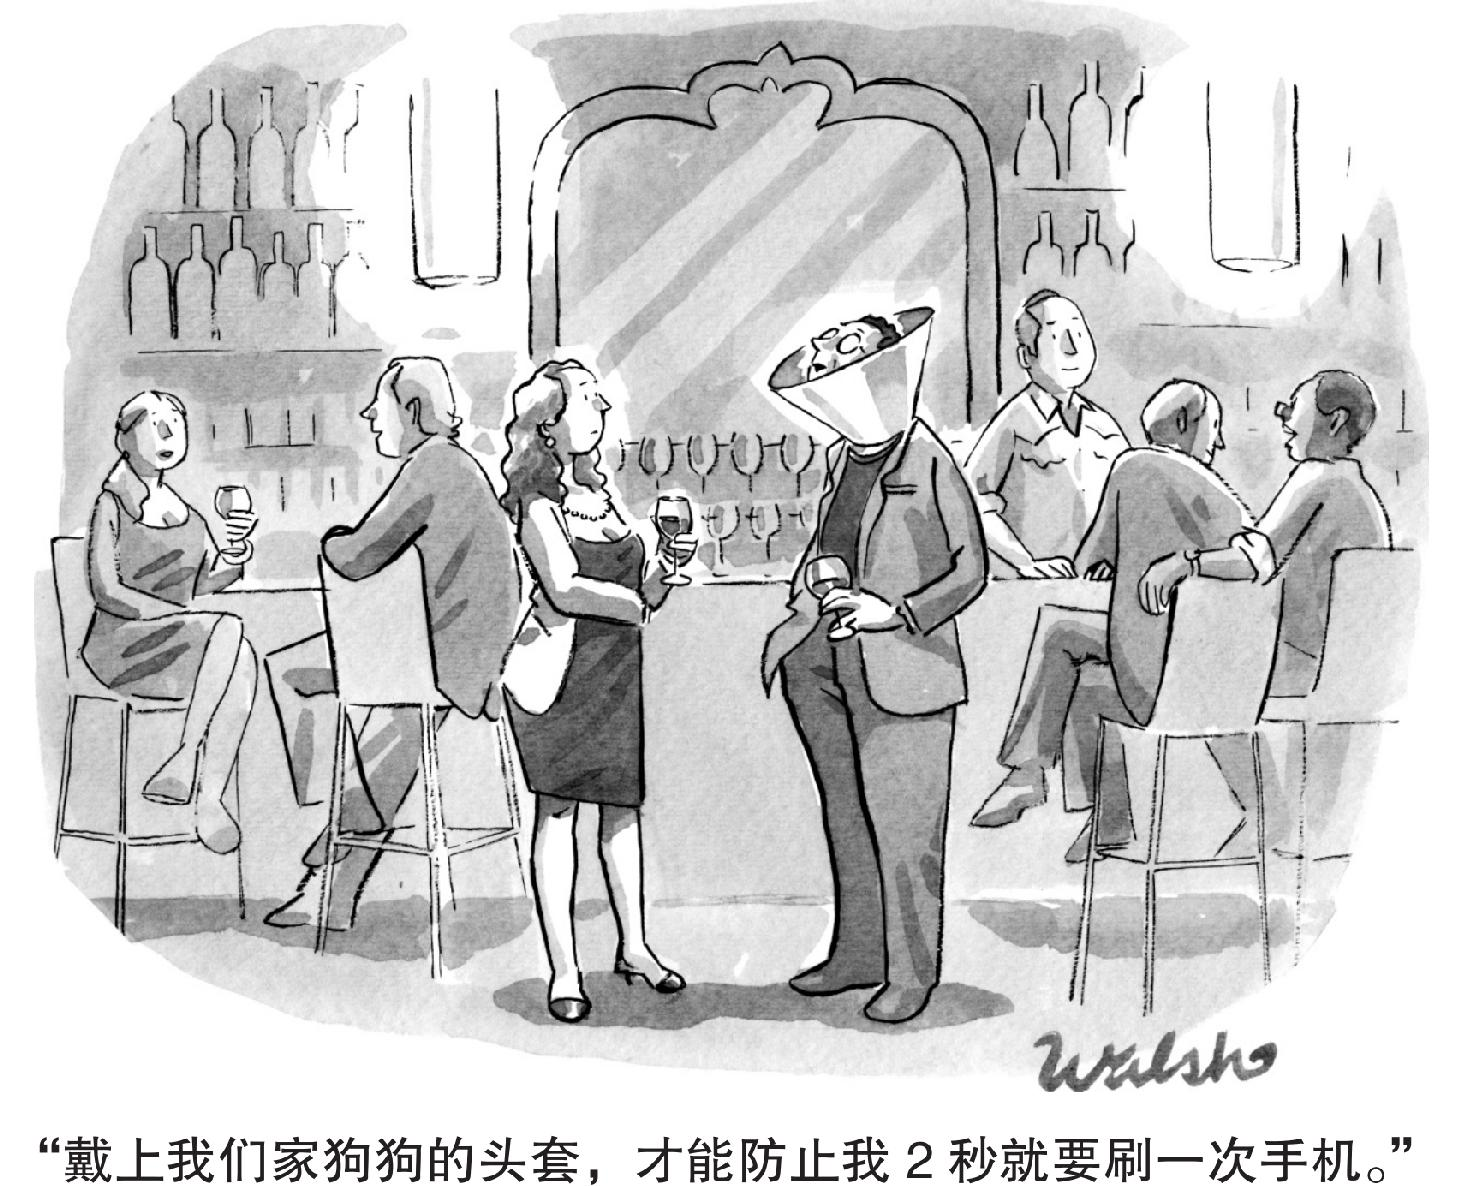
\includegraphics[width=0.78\linewidth,keepaspectratio]{image/44-1.jpg}
\caption{}\label{fig:44-1}
\end{figure}

每天，事情都在变得更好、更快。“未来肯定要比你想象的好得多。”我的好朋友彼得·戴曼迪斯说。他是X大奖基金会的创始人、太空飞船设计师、医生、实业家，是一个伟大的全才。“现在人类正在进入彻底变化的时代，科技有潜力提升每个人的基本生活水平，包括每个男人、每个女人、每个孩子。”

这对于你来说有什么意义呢？这意味着即使你搞砸了，并没有照着你在本书前面章节里学到的投资理财方式去做，存的钱很少，赚的钱也很少，也没关系，未来你还是能够享受到相当好的生活，远远超过你的想象，即使你将来并没有一份巨额收入也不要紧。对于那些听从了我前面的投资理财建议会有一大笔收入的人来说，未来你有无限的可能，未来的生活好得远远超出你的想象。

\begin{BookQuote}
富有的关键是用有限的环境满足无限的想法。

\hfill ——玛丽安·威廉姆森
\end{BookQuote}

科技将会改变我们对短缺的看法。短缺，是让我们感到恐惧的一个共同因素。我们害怕我们需要的东西数量不够，或者我们觉得非常宝贵的东西数量不够，包括饮用水、食物、金钱、资源、时间、空间、快乐、爱。为什么大家都想变得富有？因为我们都相信，一旦自己变得富有，就能得到足够的东西，再也不会因为缺少自己想要的东西而发愁。“这种恐惧，我们脑子里天生就有。”

但是短缺并不一定是永久的状态。科技会改变短缺情况。你知道吗？有很多年，地球上最短缺最宝贵的金属是……难道是铝？对了，你猜对了！起初要把这种元素从泥土中分离出来非常困难，花费非常大。结果当年铝以稀为贵，在19世纪的法国，拥有铝制品是最高地位的象征，在国宴上，拿破仑三世招待泰国国王用的是铝制餐具，而不是常见的金制餐具。但是到了19世纪末，科学家经过几十年的探索研究，找到了电解铝的工艺，使铝可以大规模生产，一下子这种又轻又便宜的金属在市场上随处可见，从此原来帝王才能用得起的铝制品走入万千寻常百姓家。

彼得·戴曼迪斯喜欢用铝的故事来说明，短缺程度取决于我们获取资源的能力，或者说是短缺程度取决于我们缺少的获取资源的能力。他写了一本非常棒的书《富足：改变人类未来的四大力量》，这本书有300多页，讲述了一些关于未来的概念，我们这一章只简略地介绍一下。这本书用了一个很棒的比喻来解释科技如何征服短缺。“想象一下，有一棵巨大的橙子树，上面结满了橙子。”彼得·戴曼迪斯写道，“如果我只是从那些很低的树枝上摘橙子，那么那些很容易够得着的橙子很快就被摘光了，橙子就变得短缺了。但是如果有个人搞了一项新的科技发明，叫作梯子。现在，使用梯子，我能够得着的橙子就变多了，橙子短缺的问题就解决了。科技是一个解放资源的好办法。”

由于全世界人口不断增长，我们需要用科技解放这些资源，速度要比以前更快。这就需要实现我们前面说过的那种指数型变化。指数型变化是什么？下面就是一个例子。

\begin{itemize}
\item 人类用了20多万年的时间，直到1804年，才让全世界人口达到10亿。
\item 接下来只用了123年，到1927年，全世界人口就又增加了10亿，世界人口总数达到20亿。
\item 但是接下来只用了33年，到1960年，世界人口就又增加了10亿，世界人口总数达到30亿。
\item 接下来只用了14年，到1974年，世界人口就又增加了10亿，世界人口总数达到40亿。
\end{itemize}

世界人口增长并没有到此停止。尽管中国13亿人口实行了“计划生育”政策，再加上全世界其他国家控制人口增长的努力，但都没有阻止世界人口的加速增长，只是最近40年，世界人口就新增加了30亿！也就是说，最近40年增加的人口数，相当于人类历史最初20万年增加的人口数量的3倍！现在地球上人口总数有72亿！照这个速度增长下去，科学家预计，到2050年地球上会有96亿人。

地球能养活这么多人吗？我们持续消耗自然资源，按照现在的消耗速度，根据《华尔街日报》上引用世界自然基金会的吉姆·利佩的研究结果：“我们现在使用的资源数量，比地球能够持续产生的资源数量超出了50\%，除非我们改变发展方式，不然这个数字还会快速增长，到2030年，即使有两个地球，产生的资源也不够我们人类使用。”

人类的独创性和科技融合在一起，才能够找到一种方式，持续满足我们的需要。

我记得有一段时间，我们以为人类要把石油用完了。那是1973年，我还是一个高二学生，当时中东发生了石油危机。年纪大的人都还记得，那时汽油实行配给制，按照车牌号，一天是单号加油，一天是双号加油。还在读高二的我心里直嘀咕：可能我还没有拿到驾照，地球上的石油就用完了，我这辈子连汽车都开不上了！有一天，在学校里，我们的工程学老师说：“我来给大家读一篇文章。”那篇文章我在《时代》杂志上已经读过了，是罗马俱乐部发表的一份研究报告，这份研究报告把每个人都吓死了，因为它预测我们的石油供应只能再持续几年，整个经济将会崩溃。老师读的这篇文章讲的内容差不多，用的也是对未来非常悲观失望的语气。然后老师给我们展示了一篇他过去读过的东西，那是19世纪50年代报纸上的一篇文章，讲的也是燃油危机。不过当时的人讲的燃油是——鲸油。

在19世纪，鲸鱼的脂肪是点灯用油的主要来源。没有鲸油，你在家里根本没有办法点灯照明。但是鲸鱼当时被过度捕杀，人们担心会出现点灯用油的短缺，结果鲸油的价格都涨到天上了。但是1859年发生了什么事情呢？在宾夕法尼亚州发现了原油。我们从此可以得到一种全新的资源。不久，我们就用上了煤油灯和内燃机。1973年的石油危机？科技已经减轻了石油短缺问题。新的石油勘探和开采技术，为石油供应量打开了更加广阔的空间，现在采用横向钻井技术，美国能够开采的天然气储量，按照油气当量计划，超过沙特阿拉伯的原油储量！这样的科学技术改变的并不只是一个国家的经济情况，而且会对地缘政治产生影响。2013年，10年来几乎第一次，美国国内生产原油的数量超过了从中东进口的原油数量。

未来还会有其他替代能源，例如风能、生物燃料，还有最大、最方便利用的自然能源——太阳能。按照发明家和未来学家雷·库兹韦尔的说法，世界上的能源需求总量，只要用地球上太阳能的万分之一，就可以解决了。捕获和储存太阳能的技术已经有了，关键是成本要降低到有竞争力的水平，这是最大的挑战。雷·库兹韦尔预测，再过几年，每瓦太阳能发电的成本就会低于原油和煤炭发电的成本。

\begin{BookQuote}
我们需要的是，有更多的人擅长解决不可能解决的问题。

\hfill ——西奥多·罗特克
\end{BookQuote}

我们停下来想一想：所有这些新科技是从哪里冒出来的？过去一直从我们大家熟悉的那些地方冒出来：硅谷、美国国家航空航天局、美国国防部高级研究计划局、世界上一流的大学和实验室。但是现在越来越多的自己动手的独立发明人出现了，他们运用网络上的丰富资源，找到方法把事情做得更快、更好、更便宜。

我给你讲一个少年儿童搞发明创造的故事。我遇到了一个小孩，自己创新设计出一个机械假肢，假肢行业掀起了一场革命，这个革命的发源地就是他的实验室，其实就是他的卧室。这个少年名叫伊斯顿·拉切贝尔，他17岁到美国国家航空航天局开展了一个机器人项目，他根本不用去上大学来学工程学，因为他有网络。

伊斯顿·拉切贝尔是在科罗拉多州一个很小的镇上长大的，那里没有什么给小孩玩的玩具。于是他在家里自娱自乐，把家里的玩具、电器之类各种各样的装置拆了又装，装了又拆。14岁的时候，伊斯顿决定自己打造一个机械手臂。为什么？好玩呗！他住的小镇上既没有大型图书馆也没有大学，于是他在网络上搜索，自学电子学、编程、机械。然后他用他身边能够找得到的东西，包括乐高积木、钓鱼线、绝缘胶带、玩具小马达，还有一个玩游戏用的任天堂能量手套，造出了一个机械手臂原型。

等到他16岁的时候，他进一步完善设计，因为这时他得到了一台3D（三维）打印机，能用一层一层的塑料打印出一个机械手臂。伊斯顿带着这个发明参加了科罗拉多州的科学展览会，正是在那里，他找到了他所说的“啊哈”时刻，他一下子顿悟了。伊斯顿碰到了一个7岁的女孩，两只胳膊装的假肢，家里花了8万元，等她长大成人还需要再装两个大的胳膊假肢。伊斯顿一听，心里说：“谁能买得起那么贵的假肢呢？”除了价钱贵之外，这个假胳膊上连的机械手功能非常有限，上面只有一个感应器，只能做一种运动。相比之下，伊斯顿设计的机械手臂装置就灵活多了，还有5个灵活的手指。就在那个地方，就在那一刻，伊斯顿决定设计创造一个新型机械手臂，使用简单，功能实用，价格便宜，大家都买得起，从而帮助那些像那个小姑娘一样失去胳膊需要装假肢的人。

伊斯顿回到他的卧室兼实验室，打造出来一个完整的机械手臂，能够复制人类手臂的动作和力量，但更加令人惊奇的是，他想出一个好主意，为手臂配一个脑电波头戴式设备，将脑电波转化成蓝牙信号，来控制这个机械手臂。（这些东西并不只是科幻电影里才有。）这个机械手臂比小姑娘花8万美元买的假肢轻1/3，力量却强大得多。事实上，一个人用这种机械手臂能提起150千克重的东西！和过去假肢的性能相比，这是多么巨大的改进。那么你猜猜伊斯顿发明的新型机械手臂成本是多少？跟那个8万美元的假肢相比，功能强大这么多，价格肯定应该更贵对不对？然而，恰恰相反，这款假肢便宜多了。2万美元？5000美元？1500美元？只要250美元！

18岁生日前那个夏天，伊斯顿受到美国总统奥巴马的接见。随后，伊斯顿到美国国家航空航天局位于休斯敦的约翰逊太空研究中心实习，由他领导一个团队研发机器人技术，用于国际空间站。到了8月底，伊斯顿就待不下去了，心里想：“我要离开这里，这些家伙做事太慢了！”他非常想制造自己设计的东西，可是这里有太多层级的官僚机构，需要一级一级批准。于是他又回到家里。伊斯顿开始打造一个机械外骨骼，这是为他所在高中的一个男孩设计的，那个男孩出了车祸，腰部以下瘫痪。伊斯顿希望他穿上机械外骨骼，能够自己行走，参加毕业典礼。

我一看到伊斯顿研发机械外骨骼的报道，就想我一定要联系上他。我一直在跟最近大规模枪击事件的幸存者一起合作，包括康涅狄格州牛顿市和科罗拉多州奥罗拉市的两起枪击事件。我帮助很多幸存者改变他们的人生，在人生蒙受如此巨大损伤之后能够重新振作起来，重新正常生活。其中一位是阿什利·莫泽，她是个怀孕的妈妈，亲眼看着那个发疯的杀人犯杀死了她6岁大的女儿，然后掉转枪口指着她。两颗子弹射穿她的肚子，杀死了肚子里还没有出生的孩子，也让她腰部以下瘫痪。我遇见阿什利的时候，她满脑子都是自杀的想法，我用飞机去接她的家人和医疗团队来参加我们“释放内在力量”的活动，我们一起努力，想要创造出一种环境，让这个可怜的年轻妈妈能够开始她的情绪治愈过程。

我很希望阿什利能够重新行走，于是我联系伊斯顿，提出要赞助他的研究计划。从那以后我们两个就开始业务合作了，想要创造发明出一种低成本的假肢装置，能够用到全世界，让很多人用了这种机械手臂，人生从此发生巨大变化，不管他们住在哪里，不管他们有多少钱，都能装上这种机械手臂。这就是伊斯顿的使命。

伊斯顿的另外一个使命是，向全世界的年轻人传播他的想法，所有年轻人都能成为高科技的创造者，而不只是消费者。“每个人都可以成为创造者。”伊斯顿说，“只要能上网，能用上3D打印技术，那么小孩子想做什么都能做到。他们不必在思想上受限于‘我必须得去上大学才能成功，除此之外根本没有别的路’，其实你真的有很多其他选择。”

毫无疑问，伊斯顿·拉切贝尔是一个非凡的人物，也许称他为天才都不为过。但是你认为世界上还有多少个伊斯顿这样的天才少年，在印度、坦桑尼亚、澳大利亚、塔吉克斯坦、乌拉圭、新加坡，天天挂在电脑上，梦想着找到办法来改善我们居住的这个世界？伊斯顿用开源的技术来分享他的第一个机械手臂设计，这样全世界的人都能够模仿、改进，只要他们愿意做就能自己做出来。现在我们所有人都可以成为自己的出版者和创造者，通过互联网，跟任何一个人来分享我们的创意。

闸门已经打开，科技创新的浪潮奔腾而来，带来我们这个时代最伟大的革命之一——人们称之为创造者革命，我们这个时代也成为创造者时代。伊斯顿·拉切贝尔，只是创新大爆炸的众多前沿人物之一，正是科技迅猛发展进步才让无数个人成为自主创新者。克里斯·安德森，3D机器人公司的首席执行官，他将此称为“新工业革命”。现在全世界的人想学什么都能学到，原来只有考上哈佛大学、麻省理工学院、斯坦福大学这些世界名校才能学到的东西，现在全世界的任何人只要上网都能学到。每个人只要上网就可以跟世界上最好的老师进行互动，而且是一对一交流，比大学里的学生上课交流更加紧密，分享想法，分享技术，制造设备，提供服务，这些东西过去要花费好几百万美元，现在只要几百美元就可以得到了。

每一年，创新者大会都会在全美各地召开，参加展会的创新者多种多样：发明者、业余爱好者、工程师、学生、教师、艺术家、企业家，他们一起来到这个“地球上最伟大的创新者秀”。2013年，全球共举办100场创新者大会，超过54万人参加。创新者传媒是创新者大会的创立者，2014年6月18日，时任美国总统奥巴马在白宫主持召开一场创新者大会。有个5米多高的机器人斑马，名字叫鲁塞尔，和总统热情打招呼。奥巴马参观了一个12平方米的可携带房子，还玩了一下用香蕉制造的键盘。奥巴马总统会见了来自旧金山的马克·罗斯，当他还住在无家可归的流浪汉收容所里的时候，他就开始到当地的科技市场学习如何使用3D打印机和激光切割机。16个月之后，他自己创办了一家激光切割企业，现在开展一个培训项目，给那些想要重新开始创业的人培训高科技实用技术。

奥巴马还公开称赞北卡罗来纳州两个十一二岁的小女孩，她俩创办了一个机器人公司，而不是像大多数同龄少年那样去送报纸。她们的座右铭是：“只要你能想象到，你就能做到，无论它是什么。”

“这句座右铭非常适合美国人。”奥巴马对观众们说，“美国是非常能想象的国家，想象用铁路连接一整个大洲，想象把电力送到所有城市和乡村，想象摩天大楼直入天际，想象用互联网让你我紧密相连。”奥巴马呼吁每个公司、大学、社区都要支持这些创新者。“如果我们这样做，我们就会创造出更多好工作，再过几年就能做到。我们就能创造出一些全新的行业，我们以前根本想象不到。”

创新革命正在逐步成为现实，推动创新革命的力量是新技术大爆炸和网络大扩张。10年之前，互联网只连接5亿人，现在互联网连接20亿人。专家估计，只要再过6年，就会又有30亿人加入互联网，那么互联网就会连接50亿人。想象一下，50亿人在互联网上，会在这个星球上激发多少新的联系，会释放多少创造力，联网的力量会有多大！最早的互联网，只是军事机构和科研院校之间联系的互联网，后来成了公司的互联网，再到后来成了创意的互联网，最后有了社交媒体就成了人际关系的互联网。现在的互联网是万事万物的互联网。电脑和感应器可以植入日常使用的物品之内，相互传递信息。机器跟机器之间互联，机器又跟我们人类互联，把所有的人所有的事物互相联结成一个强大的全球性网络。3D打印技术正好是一个代表性技术，可以说明这种互联网会如何改变和扩张，远远超越我们最狂野的梦想。

\subsection{3D打印：从科幻小说到科学现实}

还记得吗，在电影《星际迷航》里，企业号飞船上有复制机，能够无中生有，把能量转化成特质，凭空合成出来汉堡包和热咖啡。不过，科学家说，我们再过不久就可以创造出真正的复制机了！我们已经讲了很多3D打印，但是你可能很难理解这是一种力量多么强大的技术，除非你亲眼看到3D打印的实况才会相信。3D打印其实是一个代表数字制造的短语，含义很广。“打印机”实际上是一个迷你工厂，用计算机文件作为蓝图，一层一层地创造出三维立体物体，3D打印机可以使用至少200种液体或者粉状材料，包括塑料、玻璃、陶瓷、钛、尼龙、巧克力，甚至活细胞。用3D打印机能制造出什么东西？更好的问题是，用3D打印机不能制造出什么东西？到目前为止，用3D打印机能制造出来的东西有：跑鞋、金项链、飞机零部件、餐具、比基尼、吉他、太阳能电池板——更不用说人的气管、耳朵、牙齿。你知道，有些3D打印机体积很小，一个小孩子的卧室就能装得下，能够把一层又一层的合成糊状物变成一个能够有效发挥功能的假肢。在中国还有一种体积很大的3D打印机，一天能够打印出来10套房子，用的是一层又一层的混凝土与可回收建筑废物的混合物。成本？一套房子只需要5000美元，而且几乎不需要劳动力。

也许更重要的是，美国国家航空航天局和“美国制作”这家3D打印公司合作，应对人类最大的挑战之一：避难所需要，特别是紧急避难所。当发生自然灾害，例如龙卷风、海啸、地震等，会一下子需要面积很大的避难所。想象一下，用3D打印机，现场打印出来房子，使用当地的材料，只用几个小时，而不是几个月就能完工，那会造福多少受灾的人。这项技术的作用，如果有效使用，简直是无限大。

有一天，也许你不用离开家门一步，就能打印自己合身的蓝色牛仔裤。与此同时，地处喜马拉雅山脉的山村，能从云端下载样式，打印出来工具、水泵、教学用品，当地人需要的东西都可以打印出来。你也可以打印出来空间旅行飞船，当然，3D打印这种新科技来了，有些旧技术就会毁灭，有些老行业可能就消失了。将来五金配件商店就没有多大的存在必要了，因为很多零件都可以用3D打印，是不是？货物运输因此也会大大减少。这对于我们的星球肯定是件大好事，但是如果你是个卡车司机，那么对于你来说情况就不太妙了。专家预测，美国350万个卡车司机会失业，因为将来会有机器人自动驾驶卡车，能够每天24小时运行，而要是人来驾驶，开上8个小时就必须休息。而且你根本不需要付给司机工资，你只用投资一辆自动驾驶的卡车就行了，司机是随车免费赠送的。

随着旧行业的消失，新的行业就会出现，我们要训练思维模式来拥抱改变，来满足新型经济的需要。

3D打印技术只是高科技中的一项而已，还有很多非凡的科技正在发展进步，将会改变你的生活品质。纳米科技、机器人、组织再生，这三项技术也非常值得关注。要是你还搞不懂为什么我们要讨论上面这些东西，我告诉你，因为我们知道，科技发展进步为我们目前很多最紧迫的问题提供了解决方案，不管未来是什么经济季节，不管我们经历通货膨胀还是通货紧缩，不管是战争还是和平，科技发展进步都会持续不断地发生。

听说过人口浪潮吗？婴儿潮一代出生的有7700万人，这一代人的消费支出推动美国经济增长了好几十年。但是现在每天都有10000个婴儿潮出生的人年满65周岁，这就形成了一种潜在的退休危机浪潮，因为他们大多数人都没有存下足够几十年退休生活支出的一大笔钱，也根本没有养老金。

有一股债务浪潮正在美国这个国家内部形成，比历史上任何时候的债务规模都要大：17万亿美元债务，还有100万亿的没有资金支撑的支付责任，包括医疗保障制度、医疗补助方案、社会保险计划，以及美国政府的其他承诺。

\begin{figure}[htbp]
\centering
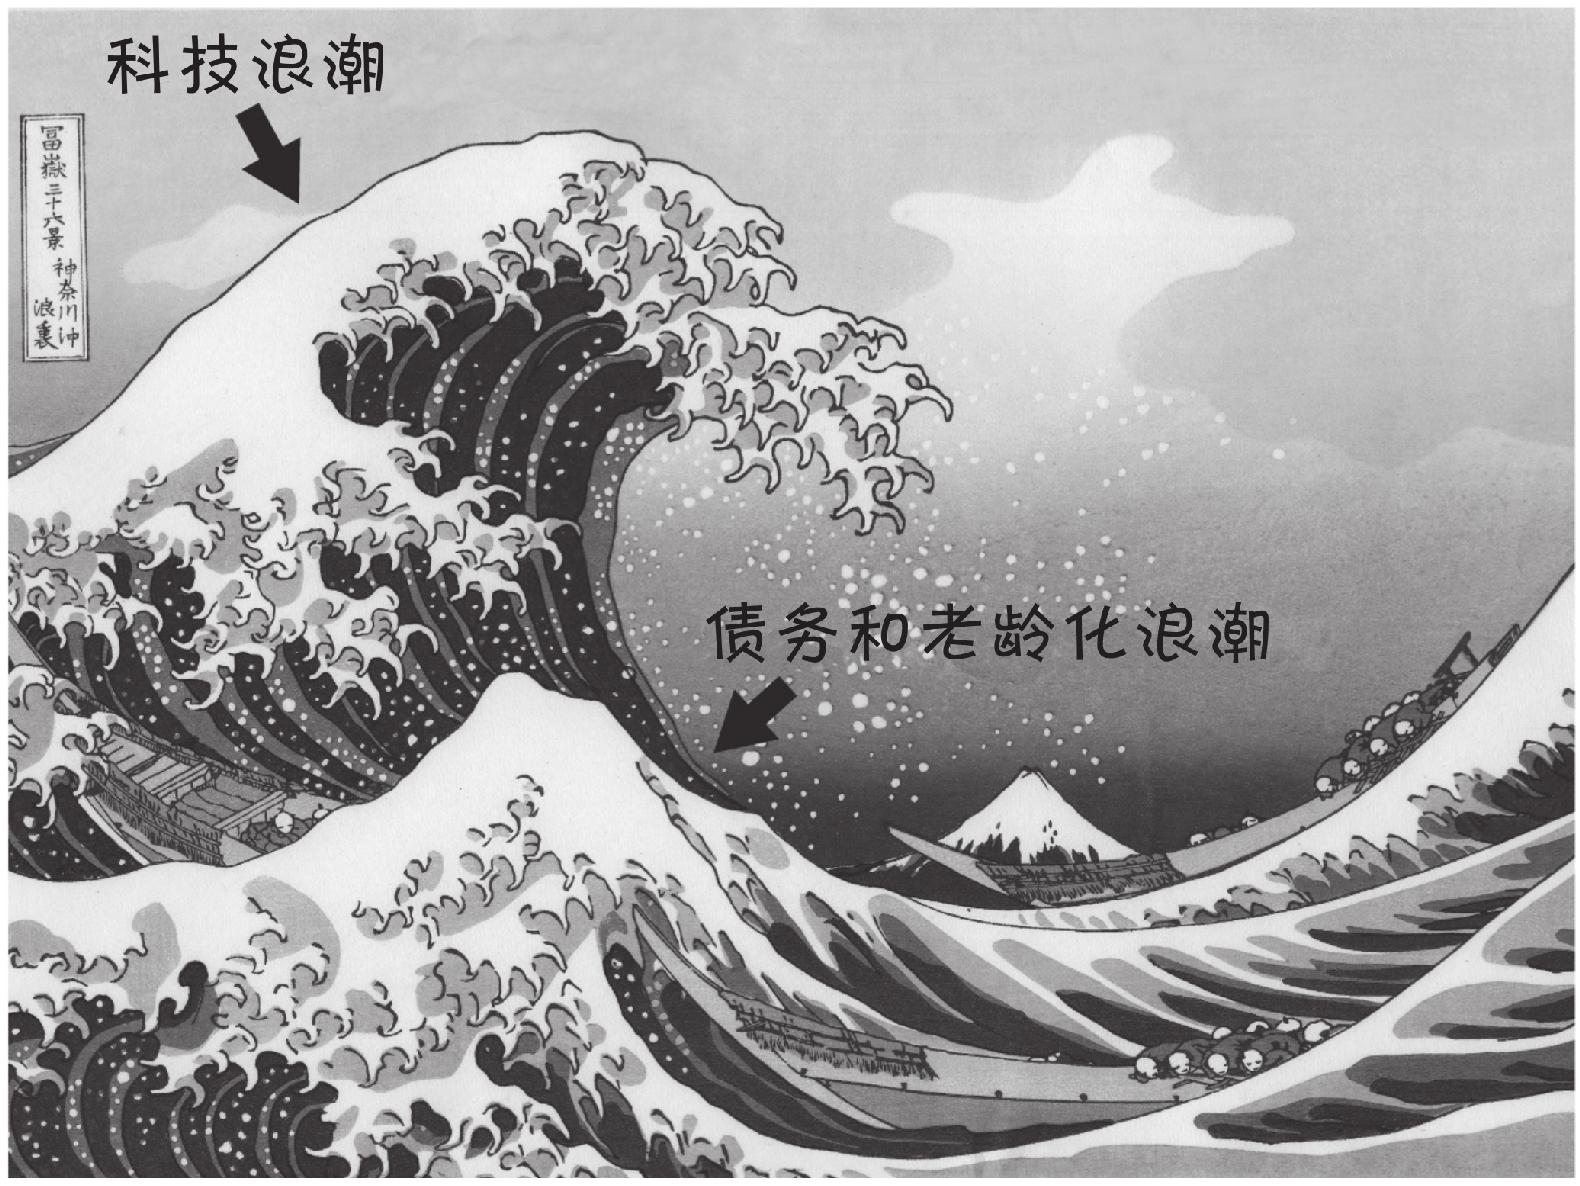
\includegraphics[width=0.84\linewidth,keepaspectratio]{image/44-2.jpg}
\caption{}\label{fig:44-2}
\end{figure}

还有一股环境浪潮也在形成，尽管可能你并不相信气候变化。但是很明显，现在我们所居住的陆地气温过高。不管人口浪潮、债务浪潮和环境浪潮有多大，科技浪潮都会更大，并承诺能让所有的船都升起，带领整个世界进入更加富足的未来。

我想这些技术的潮流倾向比任何问题都重大，那是在我最近举办的一次经济研讨会上，未来学家和风险投资家胡安·恩里奎斯说，尽管每个人都担忧朝鲜战争和冷战，但那时人们还是发明了晶体管，尽管每个人都担忧“二战”，人们还是制造出了抗生素。大多数这些进步，都对你的生命有更加重要的影响，影响比战争还要大，比那些政治和经济的起起伏伏还要大。

我们的问题一波接一波地冒出来，但是解决方案也一波接一波地冒出来。

\begin{BookQuote}
我在巨大的生命浪潮上冲浪。

\hfill ——威廉·夏特纳
\end{BookQuote}

科技创新像波浪一样呈指数型增长，对于这个看法的了解，没有能胜过我的好朋友雷·库兹韦尔的，他是个发明家，又是作家，又是企业家。作为我们这个星球上的最强大脑，大家称他为我们这个时代的托马斯·爱迪生。不过你可能从来没听说过他的名字，除非你是一个特别喜欢收看TED演讲的人，或者你研究过谷歌的团队成员组成，你才知道他是谷歌工程设计部门的头儿。不管你是否知道他这个人，雷·库兹韦尔在很多方面都影响了你的生活，比你能想象的还要多得多。你用手机播音乐，或者用电脑播放网上的音乐，或在任何地方听到数字设备播放出来的音乐，你都要感谢这个人——是他发明了第一首数字音乐。如果你用Siri（苹果手机上的语音控制功能）语音输入一封电子邮件，或者用的是语音转换文字系统，那么你要知道这些发明都是雷·库兹韦尔的功劳。

我记得，大约20年前，我第一次听到雷·库兹韦尔描述的未来，我很震惊，这听起来好像是魔法一样遥不可及，但是现在都成了现实，就在身边：汽车自动驾驶；电脑可以击败世界上最厉害的象棋大师。雷·库兹韦尔发明了光电符号识别系统，就是我们常用的扫描文字识别，给盲人创造出来第一个阅读机器，歌手史蒂夫·汪达是他的第一个客户。现在他想帮助盲人识别街道标志，在城市里自主穿行，不需要别人的帮助，进入餐馆可以自己“看”菜单点菜，只用一个香烟盒大小的装置就行了。雷·库兹韦尔告诉我这一切发生的准确年份是：2005年。

“现在是1995年，你怎么知道10年之后能够实现呢？”我问他。

“你不明白，托尼。技术是能够自己喂养自己的，技术发展进步会变得越来越快。技术发展进步是指数型增长的。”

雷·库兹韦尔给我解释了技术进步的摩尔定律。最初是摩尔发现计算机处理能力每两年就会翻1倍，而成本以同样的速度下降，每过两年下降一半。但是后来人们发现，摩尔定律不仅仅适用于电脑芯片，还可以应用到所有的信息技术上，最终可以扩大应用到我们生活的所有方面。

这意味着什么？有些东西不是线性增长或者代数模式增长（1、2、3、4、5、6……），而是指数型增长（1，2，4，8，16，32……），所以你会看到增长速度变得越来越快。但是我们发现，这个概念难以理解，因为这不符合人类天生的思考方式。

“首先，指数型增长跟我们的直觉有很大的不同。”雷·库兹韦尔说，“我们对未来有一种直觉判断，像在我们大脑结构定型一样，我们会自动这么想。1000年前，当我们穿过非洲的草原，从眼角看到有一个动物冲着我们跑来了，我们可以做出线性预测，再过20秒，这些动物会来到什么地方，我们应该怎么应对，逃跑还是战斗。但是如果那个动物的速度是呈指数型增长的，一开始很慢很慢，逐步加速，然后突然之间一下子就到了另一个地方。”

彼得·戴曼迪斯用另一个比喻解释指数型增长：“如果我告诉你‘走线性30步’，你走30步一般就是30米远。但是如果我告诉你‘不是走线性30步，而是走指数型30步’，猜猜你能走多远呢？10亿米，你能猜得到吗？这相当于绕地球26圈。”

雷·库兹韦尔说，明白了指数型增长，就可以预测出增长的轨迹。他知道，什么时候科技进步会追上他的展望。他预测到了他的第一个盲人用口袋型阅读器和其他产品的投放日期。雷·库兹韦尔经常在我组织的论坛活动上发表演讲。最近一次他在演讲中告诉我们，他是如何准确地预测到人类基因计划全部完成的时间的，这可是我们这个时代一个不可思议的发现。

“在1990年人类基因计划刚刚开始的时候，我就预测人类基因计划会在15年内完成，因为我意识到这个进程将会是指数型的。”但是那些怀疑的人认为需要100年才能揭开复杂的人类基因密码。过了7年半，到了1997年，人类基因计划只完成了1\%。雷·库兹韦尔说：“那些怀疑的人变得更有理由怀疑了，他们说‘我告诉过你，15年肯定不行。现在一半时间过去了，才完成了1\%。这真是非常失败’。”但是雷·库兹韦尔指出：“这并不是失败，这完全是按照计划正常进行！”指数型增长一开始速度很慢，你会怀疑，这些小小的数字能行嘛，看起来好像什么增长也没发生一样。但是等你实现了1\%，你离百分之百地完成只差7次翻倍了。人类基因计划在2003年成功完成，比预测的2005年提前2年。

那么，接下来还会有哪些重大的技术进步？我们前面讲了，如何用组织细胞让病人重新生长出自己的皮肤，没有痛苦，也没有疤痕，还有我们如何能够征服太阳能和风能，未来给我们提供丰富的能源。但是我们面临的其他巨大挑战是什么？

缺少淡水是地球上干旱地区疯狂增长的人口最关注的问题。现在全世界到处都缺水，从加利福尼亚州的洛杉矶到尼日利亚首都拉各斯，按照联合国的统计，全球每年有340万人死于水源性疾病。但是从澳大利亚到沙特阿拉伯都在开发新的脱盐技术，把海水变成自来水。以色列有一家公司叫“水创”，研制出一种机器，能从空气中提取出来干净的水，使用2美分的电力，就能产生出1升水。在偏僻遥远的村庄，没有电力，可以使用新型水塔，运用自身的独特造型和自然材料，就可以抽出空气中的潮气，把潮气转化成饮用水。

令人震惊的发明家迪恩·卡门发明了赛格威平衡车，从此名扬天下。迪恩·卡门跟可口可乐公司合作为全世界提供干净的饮用水。用一台能效很高的机器（大小跟集体宿舍用的冰箱差不多）把脏水蒸发，然后变成又干净又安全的饮用水。这家公司给这台机器起名叫“弹弓”，人类像戴维一样小，问题像巨人歌利亚一样巨大，但是解决方案像戴维的弹弓一样，虽然很小却能让戴维战胜歌利亚。有了上面这些创新，不久之后，人类用水短缺的问题就会得到解决。

雷·库兹韦尔说，新的食品技术正在涌现出来，会克服人类在食物方面面临的两大挑战：可以耕种的土地太少，农业污染太严重。怎么解决呢？改用横向种植，而不是垂直种植。雷·库兹韦尔展望未来15年会是这样的：“我们种植植物不是像现在这样用竖直方法，而是在水平方向，而且我们可以不用屠宰动物就能有肉吃，就是试管内克隆肌肉细胞，在计算机化的工厂生产肉，所有这些生产，成本非常低，但营养价值很高，对环境也不会产生影响。”不用杀虫剂，也不会因氮肥施用太多而造成污染。没必要杀死动物来获得蛋白质。这听起来简直不可能，但是库兹韦尔说，这是真的，就快要实现了。

这些人类的基本需求得以满足之后，人类就有机会实现自己更多的抱负，特别是如果我们能战胜另外两大挑战——健康和衰老。雷·库兹韦尔相信我们也能够解决这两个挑战。这样的话，人类的自由就大多了，能够自我实现的地方就大多了。

\begin{BookQuote}
年龄，是个思想的问题，而不是物质的问题，如果你根本不在意，年纪就根本不重要。

\hfill ——马克·吐温
\end{BookQuote}

我们谈论的这些变化都是革命性的，但按照胡安·恩里奎斯的看法，科学技术进步带给未来健康医疗保护的变化比别的方面更让你震惊，生命其实就是信息技术。怎么会是这样？好了，我们都知道，我们的基因就是4种化学基质构成的序列，编码分别是A、C、T、G。还记得小学生的生物作业吗？换句话说，生命本身的构件可以用代码来表示，而这些代码是可以改变的，也可以创造出来新的代码。就像制造出来人工生命一样，这正是克雷格·文特尔这位人类基因研究先锋2010年就做到了的事。胡安·恩里奎斯也是这个团队的成员。

最近在我组织的一次大型论坛上，我邀请胡安·恩里奎斯发表了演讲。我问他：“你和克雷格·文特尔是怎么想出来创造人工生命这个主意的？”

他呵呵一笑，说：“有一天，我们一大堆人在弗吉尼亚州一家酒吧里喝酒，喝了第四杯威士忌之后，有个家伙说：‘如果你能从一无所有利用编程设计出一个细胞，就像你从一无所有利用编程设计出一个计算机芯片一样，那会多酷啊？这样做需要什么？’”他停了一下然后说：“这只需要5年，投入3000万美元，就能设计出来。”首先他们从微生物里提取所要的基因，然后再植入一个新的基因代码，这个微生物就变成了一个完全不同的物种。与此同时，这是一个新的生命形式，有个网址就嵌在他的基因代码里。正如克雷格·文特尔宣布这项惊人的颠覆性创新时所说的：“这是我们这个星球上第一个自我复制的物种，它的爸妈是一台电脑。”

雷·库兹韦尔解释道：我们的记忆就像软件程序一样，可以改变，从而像控制开关一样开始或者结束人的行为。这意味着什么？在未来我们可以用细胞做一个小机器，对它们编程来制造其他东西，包括自我复制出更多和它们自己完全相同的东西。“这种软件可以制造出自己的硬件。不管我如何把一台ThinkPad电脑编程，第二天早上我也还是只有一台ThinkPad，但是如果我把一个细菌进行编程，第二天我就会有10亿个细菌。”胡安说。

这听起来很疯狂，好像科幻小说里才会有的东西，我只能一再提醒自己，这不是科幻小说。这种技术已经用来制造衣物。“你现在穿的适合的、有弹性的衣服，像安德玛这个牌子的运动服，是吧？”胡安说，“现在所有这样的衣物，都是用细菌制造出来的，而不是用石化产品制造出来的。”在日本，用细菌培养出来的合成丝绸比钢铁还要强韧。农场里饲养基因改变过的动物，已经用来作为医疗工厂。在新英格兰有这样一个牧场，那里的牛奶可能能够治疗癌症。

\begin{BookQuote}
人的头脑能够感觉到并相信能做到，人就真的能做到。

\hfill ——拿破仑·希尔
\end{BookQuote}

我告诉过你，这是一个全新的世界，你会踏上一个狂野之旅。纳米科技和3D打印技术的进步，意味着将来会有一些医疗设备像血细胞一样小，有一天可能会在你的身体内游走，来和帕金森病和阿尔茨海默病这样的疾病做斗争。纳米量级的计算机插入物将会替代那些疾病摧毁的生物神经细胞。使用微型耳蜗植入物，不但可以恢复人的听力，还可以提高人的听力，让人类能听到的频率像鲸鱼歌唱的频率一样广。按照雷·库兹韦尔的说法，现在有些工作已经完成了，能创造出基因强化血液红细胞，有一天能够携带足够多的氧气，让潜水员吸一口气就能在水下持续待上40分钟，用在战场上就能挽救受伤严重的战士的生命。

现在科学家正在研究，使用3D打印机创造出量身定做的器官和其他身体部位，及时满足你的需要，从而消除危险又昂贵的捐赠器官移植。安东尼·阿塔拉医生是苏醒森林再生医药研究所的所长，他说：“从理论上，任何体内生长的东西都能够在体外生产出来。”阿塔拉医生在实验室里创造出有完全功能的人造膀胱，并完成了移植。最近15年，从干细胞生长出来的人体组织，移植后没有一例受到身体排斥。阿塔拉医生和其他人正在努力培育更加复杂的器官，像心脏、肾、肝。也许将来某天，如果你得了心脏病，或者你的心脏瓣膜受到病毒损坏，你的医生可以为你定制一个一模一样的新的心脏瓣膜，或者可以用你的一些皮肤细胞，为你培养出一颗新的心脏。

如果你财力足够的话，有些奇迹般的治疗手段现在就能使用。有一种东西叫作“细胞外基质”（ECM），是用猪膀胱上的细胞做的，可用于受到伤害的人体组织上。这个母体能吸引我们自己的干细胞，再长出来肌肉、肌腱甚至骨头。现在已经用这种母体再生出手指了！这种非凡的物质现在已经存在，但是费用很高，还不是每个人都能用得起的。但是，很快就可以了。

再生医疗背后的概念非常简单：我们的身体知道如何再生出自己的各个组织器官，我们只需要知道如何启动这些就在我们体内的干细胞，使其开始生长就行了。我们知道，乳牙掉了没关系，会再长出一口新牙。但是你能想到手指也会再生吗？根据匹兹堡大学斯蒂芬·贝狄拉克博士的研究，一个新生婴儿如果失去一根手指，那么在原来的位置，过两年就会再生出一根同样的手指。随着年纪增长，人就失去了这种组织再生能力，所以问题就是我们怎么刺激出来这种再生能力。蝾螈能够重新长出尾巴，为什么人类不能重新长出四肢或脊髓？如果我们找到办法能够完全掌控干细胞的所有能力，那么它在医疗和整形美容的应用前景将会无限大。

雷·库兹韦尔说，如果我们想要以后充分利用这些医疗技术上的突破创新延长寿命，那么我们最好现在就要照顾好自己的身体。这个想法其实就是要让自己活得足够长，能够活到技术实现的那一天。如果你是2000年之后出生的“00后”，你应该会享受到这些创新医疗技术的好处。如果你是婴儿潮一代出生的人，现在已经50多岁了，你最好赶紧去买个椭圆机开始健身，还要开始合理饮食，好好爱护你的身体，让自己活到人体器官再生技术实现突破的那一天。雷·库兹韦尔甚至和一位保健医生合作写了一本书《超越：迈向生活永生的9个步骤》，告诉大家一些方法保持身体健康，利用医疗技术突破的力量，大大延长你的寿命。

雷·库兹韦尔最近的目标是，至少活到看到电脑变得比人脑更聪明的那一天。这一天很快就要到来了。

\subsection{把人脑变成电脑}

人类要花好几个小时才能吸收理解的东西，电脑只用几秒就可以做到。但是到2020年，按照雷·库兹韦尔的说法，一个1000美元就能买到的电脑，能力完全比得上人类的大脑。到2030年，一台电脑就能处理的知识相当于地球所有人类大脑掌握的知识总和。

到那个时候，我们就辨别不出人类智能和人工智能之间有什么差别了，雷·库兹韦尔说。但是我们没有什么好害怕的。为什么？因为那时的电脑就成了我们人体的一部分，让我们更聪明，更有力，更健康，更快乐。你觉得这种事情不可能发生吗？要是你的手机不在身边，你会有什么感觉？有点儿失落，是吧？这是因为科技还有依附于它的互联互通，已经成了我们生活的一部分。手机成了我们的“外置大脑”，因为手机成了我们的便携记忆中心，储存了我们太多的个人信息，导致我们根本离不开手机。未来20年，我们也许会从移动手机发展到可穿戴设备，再发展到可植入设备。

所以你可以想得更远一些。想象一下未来会是这样的世界——你根本不需要读书，你可以把本书的内容下载到你的大脑里。哈哈，我怀疑你希望这种技术现在就能成为现实，特别是你要阅读这么厚的一本书，要是能把它一下子下载到大脑里该有多好啊。你还可以想象这样一个未来的世界，你可以把你的思维、你的想法、你的个性，上传到云端，永久保存。到了这个时候，大概就是雷·库兹韦尔和其他伟大的思想家和未来学家相信的人和机器融合的时代了。这个史诗般的时刻被称为“奇点”，这可是让那些技术宅男狂喜的时刻。这种事情什么时候会发生？雷·库兹韦尔预测，奇点会在2045年左右到来。

\begin{BookQuote}
那些知道“为什么”活着的人，遇到千难万险，都能承受。

\hfill ——维克多·弗兰克尔
\end{BookQuote}

如果科技解决了我们资源短缺的问题，我们就会更加安全，更加自由，更加快乐吗？肯定是的。正是资源短缺激发出人类的生存本能，激活了人类爬虫脑的深层部分，它让你相信，这些东西要么是你的，要么是我的。这种不战即逃的机制，能帮助我们活下来，但是也会带来人类“文明”社会最坏的一面。我们现在拥有的大脑，有200多万年的进化历史。而大脑进化并没有那么大的提高，所以侵略和战争总是人类的挑战，但是资源短缺减少，引发暴力攻击的事件也就减少了。

统计数据表明，能得到更多的科学技术，会让人更快乐。世界价值调查表明，1981—2007年，调查覆盖的52个国家中，有45个国家幸福指数提高了。这是因为什么？你猜对了，就是数字革命。科技的浪潮向全世界扩散，这个报告称其为“从工业社会到知识社会的转型”。社会科学家如此解释这种幸福指数的增长：“经济发展，民主化，提升社会容忍度，这三个因素增加了人们感觉自己拥有自由选择的程度，相应地带来全世界范围内人们普遍感到幸福水平更高。”同样也是这个调查表明，拥有更多的钱并不能让人更快乐，有些最快乐的人反而生活在最贫穷的国家。生活在菲律宾的人就觉得自己比生活在美国的人更快乐。快乐更多地与价值相关，而不是和国内生产总值相关。

我们都知道，那些维持生存的劳动，剥夺了我们最宝贵的商品——时间。还记得我前面说过，不久之前，大多数美国人还都是农民，80\%的时间花在种地上，不种地就没有饭吃；现在我们每天的时间，用来赚钱得到足够食物养活自己的时间只占7\%。有了更多科学技术的帮助，我们就能有更多的自由时间，这意味着我们就有更多的机会学习、成长，与人沟通、给予，所有这些追求都让我们作为人类能够更加圆满地实现自己，成就自己，满足自己。

我们得到更多的自由时间，有利也有害。不利的那一面是：

人工智能和自动化设备将会承担越来越多由人来承担的任务。牛津大学的一项研究发现，现在美国劳动力市场上47\%的工作，未来有机械化的危险。实质上牛津大学专家的意思是，现在所有的工作，有一半都将由机器人完成，也就是有一半人会失业！这意味着，我们整个社会必须重启，给每个人创造出有意义的工作，也就是说，我们每个人都必须学习掌握新的技能。这会是一个困难的转型，这一点毫无疑问，但这是必须完成的。

但是，如果将来工作本身都消失了，由电脑来完成所有的工作和大部分的思考，那么会发生什么样的情况？我们人类要做的就是，坐在自动驾驶的汽车上到处逛，每天等着无人机送来快递。没有压力就没有动力，没有挑战就没有进步，我们什么压力都没有，也就没有相应的推动力了，那可怎么办？这是一个很有趣的问题。

十多年前，我和雷·库兹韦尔讨论过这个问题，他给我讲了一个故事。那是他小时候看的电视剧《阴阳魔界》，这是一个很有趣的系列电视剧，每一集最后总是会有一个令人毛骨悚然的转折，其中一段情节是：有个人爱赌博，死了之后，又醒来了，看到一个友善的“向导”，穿了一身白色的制服，站在他的旁边。这个向导是个天使，更像一个男管家，带他来到一个豪华的赌场，这肯定是赌徒才会想象出来的天堂。他领着这个赌徒进入一个超级豪华的包间，这个赌徒打开橱柜，发现里面都是超级奢侈的西服套装，还有超级高档的鞋子，这些衣服和鞋子穿上去都很合身，效果非常好。他的向导打开一个抽屉，里面装满钞票，比他以前看过的所有钞票加在一起还要多得多。于是这个赌徒穿戴打扮好，走到楼下，来到赌桌旁坐下，每个人都知道他的名字，每个人都对他微笑。许多比超级模特还要性感、还要迷人的漂亮女人围着他。帅气、多金、受人尊重、美女围绕，这是他的人生终极梦想，现在全都有了！开始赌吧！这个赌徒开始玩21点，第一把就拿到了21点。这简直太棒了！他一下子搂过来桌子上的筹码，心想：都是我赢的啦！第二次，又是21点。第三次，还是21点。连续十次，他都拿到了21点！这简直太棒了！这个赌徒又去玩骰子，还是赢赢赢！他赢了大量筹码。赢了这么多，当然得花了，随意点更多的酒、更多的牛排、更多的女人。想要的一切都有了。玩好、吃好、喝好后去睡觉了……我们都知道，他肯定不是一个人睡的，他这一夜过得非常开心。

以后的日子天天都是这么幸福快乐，想要什么就有什么。就这样过了一天又一天，几个月后，他又去玩21点，那个发牌的庄家说：“21点。”

这个赌徒大叫：“当然是21点。”

庄家说：“21点，你赢了。”

“当然是我赢了！我总是赢赢赢！，我都烦死了！我每次都赢，不管什么时候都是我赢！”这个赌徒大声抱怨，看着那个给他当向导的白衣天使，他要求跟天使的首领对话。

天使的首领来了，这个赌徒开始长篇大论地大声指责抱怨：“我都烦死了，我都要疯了！你知道这是怎么回事吗？肯定有什么地方出错了。我不是那么好的人，我肯定来错地方了。我根本不配住在天堂里。”

这个天使首领脸上的微笑突然凝固了，他说：“你怎么知道你是在天堂？”

如果我们不费吹灰之力，就得到我们想要得到的所有东西，那么会发生什么情况？过了一阵子，我们就会觉得像是身处地狱一样难受，是不是？这样我们就会面临一个新的问题：生活在一个物质极大丰富的世界，我们到哪里能够找到活着的意义？所以，也许到了将来你的问题就不是短缺了。解决方案并不只是物质的极大丰富。正如彼得·戴曼迪斯所说的：“物质上的极大丰富，不能提供给地球上的每一个人极其丰富的人生，而是提供给所有人拥有无限可能的人生。”

所以，在最后这几章，让我们来看一看，能给你人生永恒意义的核心是什么。有些东西能给你带来快乐，不管你是面对巨大的挑战，还是面对非同寻常的机会；有些东西能够成为你力量的源泉，不管是在经济困难时期，还是在物质极大丰富时期。让我们揭开成就和意义的终极财富，让我们学会使用激情的财富。
